In questo primo esperimento si vuole valutare la caratteristica di trasferimento del circuito bistabile mostrato in Figura \ref{fig:Circuit1}. In cui il segnale $v_i$ è applicato mediante il generatore di funzione e l'uscita $v_o$ è connessa all'oscilloscopio.
\begin{figure}[H]
    \centering
    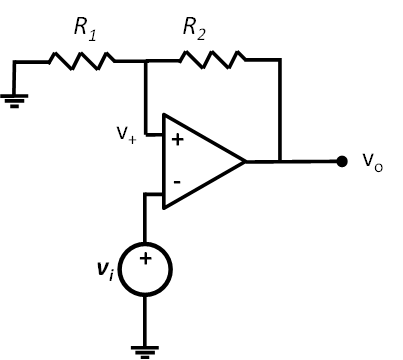
\includegraphics[width=0.4\linewidth]{images/Circuit1.png}
    \caption{Schema circuito}
    \label{fig:Circuit1}
\end{figure}
Il circuito è alimentato dalla tensione duale: $\pm V_{CC}=\pm 10V$. L'integrato TL082 contiene due amplificatori operazionali e i pinout dell'integrato sono stati ricavati dal datasheet e sono riportati in Figura \ref{fig:IC1}
\begin{figure}[H]
    \centering
    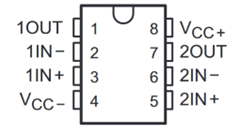
\includegraphics[width=0.3\linewidth]{images/IC1.png}
    \caption{Pinout dell'integrato TL082}
    \label{fig:IC1}
\end{figure}
\subsection{Definizione dei valori di $R_1=R_2$}
Tenendo conto delle resistenze di ingresso e uscita dell'integrato; si è scelto il seguente valore per le resistenze della rete di retroazione positiva
\begin{equation*}
    R_1=R_1=10k\Omega
\end{equation*}
Con tali valori si prevedono le seguenti soglie per il circuito bistabile
\begin{table}[H]
    \centering
    \begin{tabular}{|c|c|}
        \hline
        $V_{TH}=$&4,5V \\\hline
        $V_{TL}=$&-4,5V \\\hline
    \end{tabular}
\end{table}
I valori delle soglie sono stati calcolati sulla base della relazione
\begin{equation}
    V_{TH}=L_{+}\beta,\quad V_{TL}=L_{-}\beta,\quad\text{con }\beta=\frac{R_1}{R_1+R_2}
\end{equation}
In cui $L_{+}\text{ e }L_{-}$ sono stati ricavati dal datasheet, applicando sempre una proporzione con l'alimentazione scelta.
\subsection{Assemblaggi e settaggi}
L'uscita del generatore di segnale è stato collegato mediante il "BNC T" sia al canale 1 dell'oscilloscopio, sia al morsetto invertente dell'amplificatore operazionale. In seguito è stato connesso il canale 2 dell'oscilloscopio all'uscita dell'operazionale, prestando particolare attenzione al raggruppamento delle varie masse. In Figura \ref{fig:CircuitLab} si può vedere lo schema dei collegamenti
\begin{figure}[H]
    \centering
    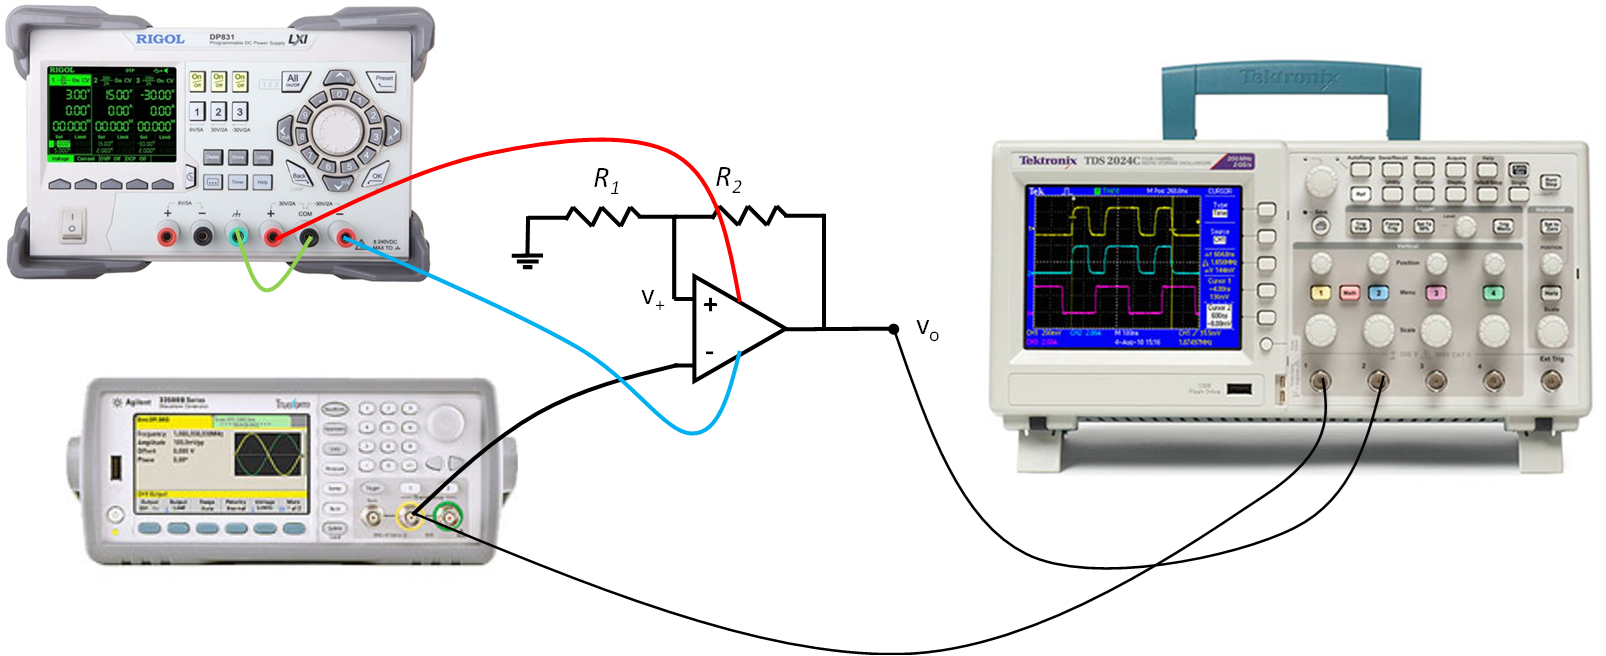
\includegraphics[width=0.8\linewidth]{images/CircuitLab1.png}
    \caption{Schema dei collegamenti}
    \label{fig:CircuitLab}
\end{figure}
Il generatore di funzione è stato impostato in modo da erogare un segnale come segue:
\begin{itemize}
    \item Forma d'onda: triangolare
    \item Frequenza: 100Hz
    \item Ampiezza: 15V picco-picco
    \item Valor medio nullo
    \item Simmetria: 50\%
\end{itemize}
\clearpage
\subsection{Risultati}
Si riporta in Figura \ref{fig:Osc1} la schermata prodotta dall'oscilloscopio che visualizza le forme d'onda in ingresso e in uscita all'operazionale
\begin{figure}[H]
    \centering
    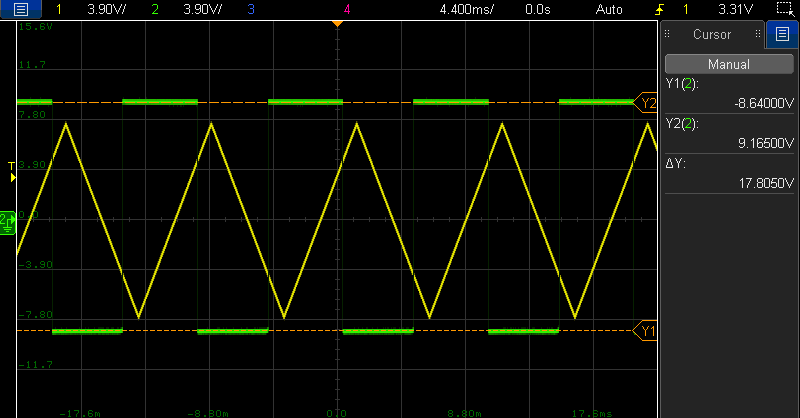
\includegraphics[width=0.65\linewidth]{images/scope_2.png}
    \caption{Forme d'onda di ingresso e uscita}
    \label{fig:Osc1}
\end{figure}
Dall'analisi dell'oscilloscopio si ricavano i valori di massimo e minimo della tensione di uscita e le soglie $V_{TH}$ e $V_{TL}$ misurate, riportati in Tabella \ref{tab:Ris1}.
\begin{table}[H]
    \centering
    \begin{tabular}{|c|c|}
        \hline
        $L_+=$&9.165V \\\hline
        $L_-=$&-8.64V \\\hline
        $V_{TH}=$&4.66125V \\\hline
        $V_{TL}=$&-4.224V \\\hline
    \end{tabular}
    \caption{Misurazioni della tensione di uscita e valori di soglia}
    \label{tab:Ris1}
\end{table}
La misura delle soglie $V_{TH}$ e $V_{TL}$ è stata fatta in modalità \textbf{xy}. In Figura \ref{fig:TrasfXY1} è riportata la caratteristica di trasferimento, usando l’oscilloscopio in modalità \textbf{xy} 
\begin{figure}[H]
    \centering
    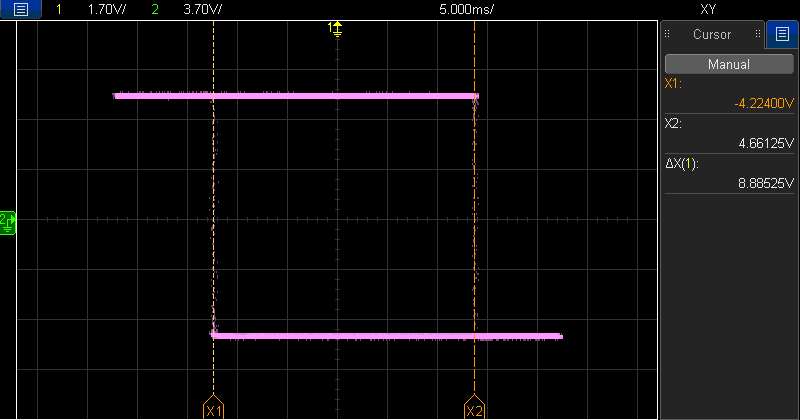
\includegraphics[width=0.65\linewidth]{images/scope_4.png}
    \caption{Caratteristica di trasferimento del circuito}
    \label{fig:TrasfXY1}
\end{figure}
\clearpage
\subsection{Risultati in configurazione Zener back-to-back}
 Al fine di limitare la corrente sui diodi al valore di $3mA$, sono stati collegati due diodi Zener back-to-back all' uscita ed è stata aggiunta una resistenza $R_3$. Il circuito è riportato in Figura \ref{fig:Circuit1.2}. 
\begin{figure}[H]
    \centering
    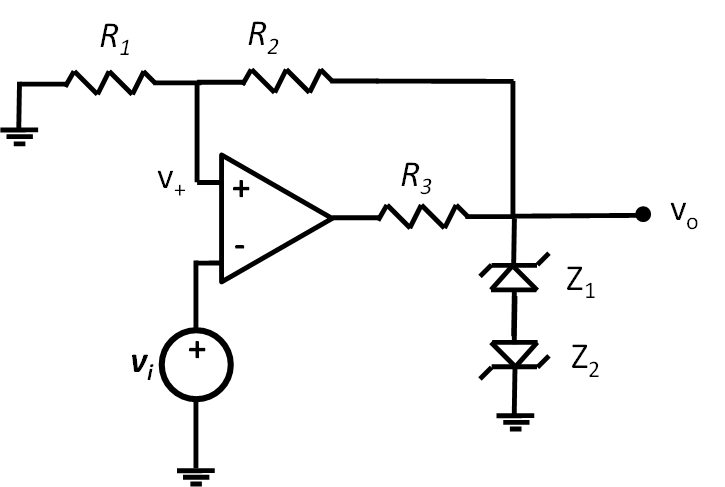
\includegraphics{images/Circuit1.2.png}
    \caption{Schema circuito con diodi Zener}
    \label{fig:Circuit1.2}
\end{figure}
Per la resistenza $R_3$ si è utilizzata la formula $\frac{L_+-V_o}{R_3}=3mA$, con $L_+=V_{Z_1}+V_D$, che ha fornito il valore $R_3=1.388k\Omega$ arrotondato al valore più vicino disponibile in laboratorio $R_3=1.5k\Omega$, in questo modo ci si aspetta in uscita la tensione di

\begin{table}[H]
    \centering 
    \begin{tabular}{|c|c|}
        \hline
        $L_+=$&+5V \\\hline
        $L_-=$&-5V \\\hline
    \end{tabular}
\end{table}
Infine viene riportata in Figura \ref{fig:TrasfXY1.1} la caratteristica di trasferimento, catturata utilizzando l’oscilloscopio in modalità \textbf{xy} 
\begin{figure}[H]
    \centering
    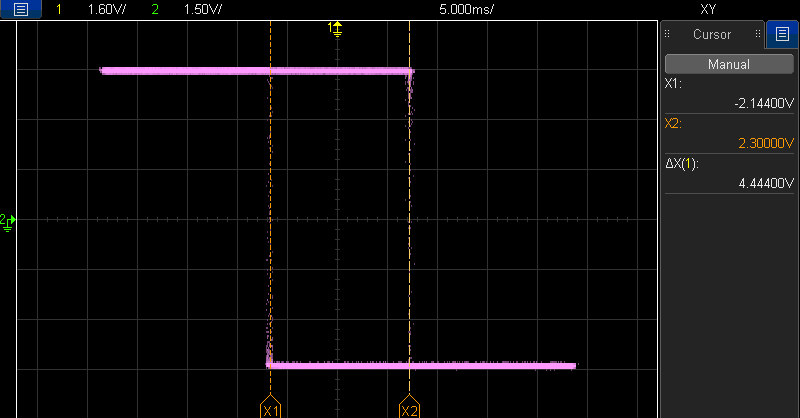
\includegraphics[width=0.7\linewidth]{images/scope_8.png} 
    \caption{Caratteristica di trasferimento del circuito}
    \label{fig:TrasfXY1.1}
\end{figure}